\subsection{Description of the model}
\label{sec:Description}


%description of the model - components and functions
We describe here a system-level model implemented to explain the hypothesis that intrinsiclly generated goals guide learning at the very first stages of sensorimotor development. 
%
The model is made of several interacting functional components.  
%
\subsubsection{Goal Generator} 
\label{sec:goal_generator}
A first component, the goal generator (GG), implements the unsupervised generation of internal categories of sensory inputs. These categories will be used in the model as abstract representations of the world that can be targeted as goals. The GG takes information from touch sensors distributed all over the body of the agent. This information is filtered so that only increments in the somatosensory activations are retained. This information about sensory saliency is further transformed so that it results in a two-dimensional retina composed of horizontally-distributed receptive fields. Figure~\ref{fig:sensory-input} shows this process. The one-dimentional body space of the agent (two arms and a line-shaped torso) is converted in a two-dimensonal touch retina. 
%
Such a retina is the input layer of a Self Organizing Map (SOM).
\begin{figure}[htp]
\centering
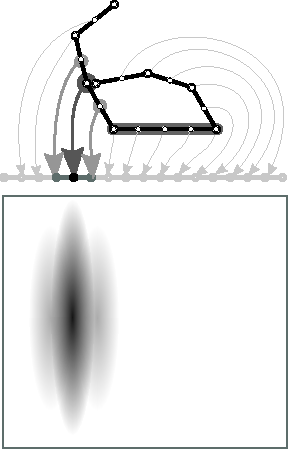
\includegraphics[scale=1.0]{sensoryinput}
\caption{}
\label{fig:sensory-input}
\end{figure}
In the current implementation the GG is a self organizing map (SOM). SOMs are a particular kind of neural network that is able to categorize all the input patterns in a given dataset in a unsupervised manner. The computation performend by a SOM is very similar to applying a k-means clustering to the input dataset. Indeed each node of the output layer of a SOM learns to detect the distance of the input patterns from the centroid of a specific cluster in the dataset. Differently from classical k-means clustering also the information about how the different clusters are distant from each other is  acquired and stored in the topology of the output layer.
% 
As we will see later, We deviate from the standard learning algorithm for SOMS in one important feature. The learning of the GG SOM is modulated by a competence-based intrinsic signal, so that both the learning rate and  the current extension of the neighbourhood (the output nodes nearby the winner that are elected for learning during each timestep) depend on the current acquired competence in reproducing the given category of stimuli instead of being preogressivelly lowered with the flow of iterations. By these means the resulting unsupervised learning is continously tempered by a motivational measure and it can cope with online streaming of input patterns.

\subsubsection{Goal Selector} 
\label{sec:goal_selector}
A second component, the goal selector (GS), implements the selection of the current goal to be pursued. In the model such a selection determines which part of the motor controller will be triggered and teached to reach the requested goal. Once the task is learned, a goal selection produces the activation of the learned skill and the reaching of the requested goal. The GS is implemented as a layer of nodes whose potentials are biased by an intrinsic motivational signal and filtered through a softmax function. As a result node potentials form a discrete probability distribution. A sample is generated at each trial from this discrete probability distribution, in which only one of the nodes is active, and this is the output of the GS. 

\subsubsection{Motor controller} 
\label{sec:motor_controller}

\subsubsection{Computing Competence} 
\label{sec:computing_competence}

\subsubsection{Computing Competence Improvement} 
\label{sec:computing_improvement}
 
\subsection{Implementation details}
\label{sec:Implementation}

\subsection{Setup}
\label{sec:Setup}